In this section we describe the new algorithm, called PaMPa-HD, proposed in this paper. Specifically, 
we describe how PaMPa-HD parallelizes the itemset mining
process and applies the pruning rules discussed in Section~\ref{Carpenter algorithm} in a parallel 
environment.
Furthermore, we discuss how, through an ad-hoc
synchronization phase, PaMPa-HD achieves a good load balancing
and robustness to memory issues.

As discussed in the previous section, given the complete enumeration tree (see Figure~\ref{running_1}), the
centralized Carpenter algorithm
extracts the whole set of closed itemsets by performing a depth first search
(DFS) of the tree.
%By tracing the set of closed itemsets encountered by traversing the tree,
%Carpenter also prunes part of the search space by applying the three pruning
%rules illustrated above. 
%described in Section~\ref{Carpenter algorithm}.
Differently, in order to parallelize the mining process, the PaMPa-HD algorithm splits the depth
first search process in a set of (partially) independent
sub-processes, that autonomously evaluate sub-trees of the search space.
%PaMPa-HD exploits the pruning rules 1 and 2 and a slight variation of the 
%pruning rule 3 discussed in Section~\ref{Carpenter algorithm}.
Specifically, the whole problem can be split by assigning
each subtree rooted in $TT|_{X}$, where $X$ is a single transaction id in the
initial dataset, to an independent sub-process.
Each sub-process applies the centralized version of Carpenter on its conditional
transposed table $TT|_{X}$ and extracts a subset of the final closed itemsets.
The subsets of closed itemsets mined by each sub-process
are merged to compute the whole closed itemset result.
Since the sub-processes are independent, they can be executed in parallel by
means of a distributed computing platform, e.g., Hadoop.
Figure~\ref{running_2} shows the application of the proposed approach on the
running example.
Specifically, five independent sub-processes are executed in the case of the
running example, one for each row (transaction) of the original dataset.
The crosses on the nodes represent the local pruning within each parallel task.
Partitioning the enumeration tree in sub-trees allows processing bigger
enumeration trees with respect to the centralized version. However, this
approach does not allow fully exploiting pruning rule 3
because each sub-process works independently and is not aware of the partial
results (i.e., closed itemsets) already extracted by the other sub-processes.
Hence, each sub-process can only prune part of its own search space by
exploiting its ``local'' closed itemset list, while
it cannot exploit the closed itemsets already mined by the other sub-processes.
For instance, Task T2 in Figure~\ref{running_2} extracts the closed itemset $av$
associated with node $TT|_{2, 3, 4}$.
However, the same closed itemset is also mined by T1 while evaluating node
$TT|_{1, 2, 3}$.
In the centralized version of Carpenter, the duplicate version of $av$
associated with node $TT|_{1, 2, 4}$ is not generated because $TT|_{1, 2, 4}$
follows
$TT|_{1, 2, 3}$ in the depth first search, i.e., the tasks are serialized and
not parallel.

Since pruning rule 3 has a high impact on the reduction of the search space, its
inapplicability leads to a negative
impact on the execution time of the distributed algorithm (see Section~\ref{Experiments} for further details).
To address this issue, we share partial results among the sub-processes.
Each independent sub-process analyzes only a part of the search subspace.
Then, when a maximum number of visited nodes is reached, the partial results are
synchronized through a synchronization phase. Of course, the exploration of the
tree finishes also when the subspace has been completely explored.
%Each sub-process analyzes only a part the search subspace, then, when memory is
%full or when a maximum number of visited nodes is reached, it stores on disk
%(e.g., in HDFS, the Hadoop distributed file system) the partial set of closed
%itemset mined so far and the remaining sub-tree left to analyze.

Specifically, the sync phase filters the partial results (i.e., nodes of the tree
still to be analyzed and found closed itemsets) globally applying pruning rule
3. The pruning strategy consists of two phases.
In the first one, all the transposed tables and the already found closed
itemsets are analyzed. The transposed tables and the closed itemsets related to
the same itemset are grouped together in a bucket. For instance, in our running
example, each element of the bucket $B_{av}$ can be:
\begin{itemize}
\item a frequent closed itemset $av$ extracted during the subtree exploration of
the node $TT_{3, 4}$,
\item a transposed table associated to the itemset $av$ among the ones that
still have to be expanded (nodes  $TT_{1, 2, 3}$ and  $TT_{2, 3, 4}$).
\end{itemize}
We remind the readers that, because of the independent nature of the Carpenter
subprocesses, the elements related to the same itemset can be numerous, because
obtained in different subprocesses. Please note that all the extracted closed
itemsets come together with the tidlist of the node in which they have been
extracted.

In the second phase, in order to respect the depth-first pruning strategy of the
rule 3, for each bucket it is kept only the oldest element (transposed table or
closed itemset) based on a depth-first order. The depth-first sorting of the
elements can be easily obtained comparing the tidlists of the elements of the
bucket.
Therefore, in our running example from the
bucket $B_{av}$, it is kept the node $TT_{1, 2, 3}$ (See Figure~\ref{running_3b}) .
The transposed tables which are not pruned in this phase are then expanded to continue the enumeration tree exploration.


Afterwards, a new set of sub-processes is defined from the filtered results,
starting a new iteration of the algorithm. In the new iteration, the Carpenter
tasks process also the frequent closed itemsets obtained in the previous iteration,
which are used to enrich the local memory of the task and enhance the effectiveness of the local pruning. 
The Carpenter tasks
process the remaining transposed tables, that are expanded, as before, until the
maximum number of processed tables is reached. In order to enhance the
effectiveness of the pruning rules related to the local Carpenter task, the
tables are processed in a depth-first order. After that, as before, in the
synchronization phase, pruning rule 3 is applied.
%A synchronization and pruning task works on the partial results
%of the sub-processes to globally apply pruning rule 3
%on the remaining search subspaces, i.e.,
%on the remaining nodes of the enumeration tree.
%After the application of the synchronization and pruning step,
%a new set of sub-processes is defined,
%for each remaining node of the enumeration tree.
%that is a descendant of one of the nodes analyzed during the first iteration a
%new process is instantiated and executed.
The overall process is applied iteratively by instantiating new sub-processes
and synchronizing their results,
until there are no nodes left.
The application of this approach to our running example is represented in
Figure~\ref{running_3}, in which the small crosses represent the pruning related to the local
state memory; and in Figure~\ref{running_3b}, in which the bigger crosses represent the pruning related to the synchronization phase.
The table related to the itemset \textit{av}
associated with the tidlist/node \{2, 3, 4\} is pruned because the
synchronization
job discovers a previous table with the same itemset,
i.e.  the node associated with the transaction ids combination \{1, 2, 3\}.
The use of this approach allows the parallel execution of the mining process,
providing at the same time a very high reliability dealing with heavy
enumeration trees, which can be split and pruned according to pruning rule 3.
Of course, this architecture cannot deliver the same pruning efficiency characterizing the centralized implementation of Carpenter in which the complete tree depth-first exploration is known.

The introduction of the sync phase leads also to a better load balancing of the tasks. At each synchronization, the tables to process are redistributed among the tasks. Therefore, the task related to the first branches of the tree, which are the ones with more nodes than others, are splitted into several subtasks. In this way, as shown Section~\ref{Experiments}, we achieve a better exploitation of the resources.


\begin{figure}[!t]
%\centering
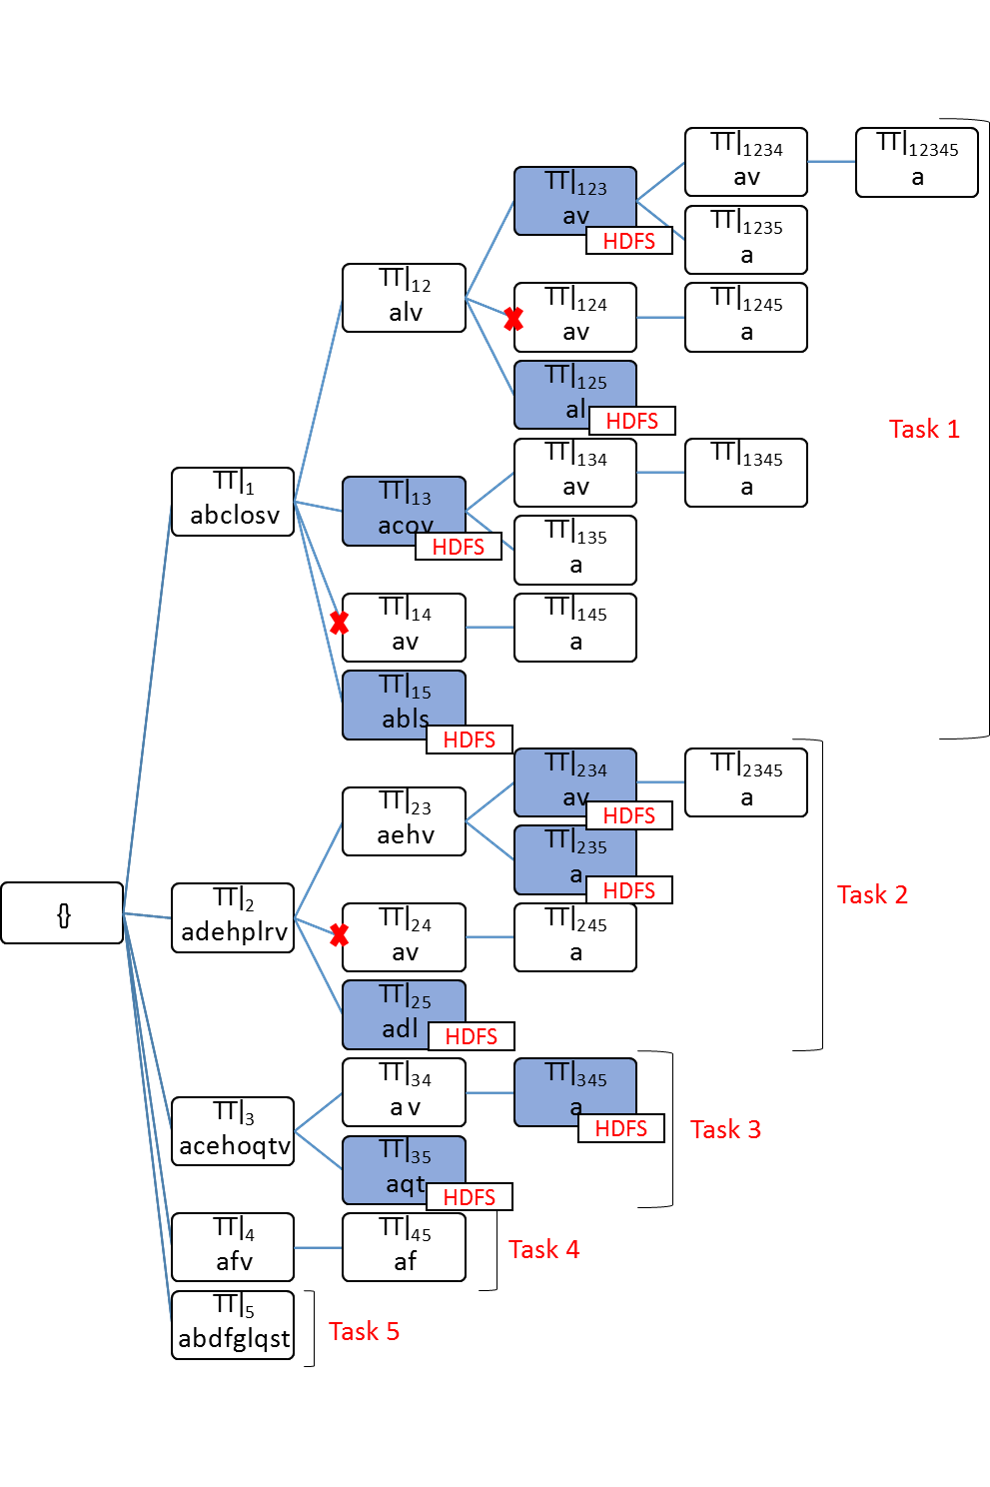
\includegraphics[width=4in]{chapters/pampa/running_example3_d_A.png}
% where an .eps filename suffix will be assumed under latex,
% and a .pdf suffix will be assumed for pdflatex; or what has been declared
% via \DeclareGraphicsExtensions.
\caption{Execution of PaMPa-HD on the running example dataset.
For the sake of clarity, pruning rules 1 and 2 are not
applied. The dark nodes represent the nodes that have been written to HDFS in
order to apply the synchronization job.}

%The red crosses on nodes represent that the nodes have been removed by the
%local pruning, e.g.,
%the one on node \{2 4\} represents the pruning of node \{2 4\}.

\label{running_3}
\end{figure}

\begin{figure}[!t]
%\centering
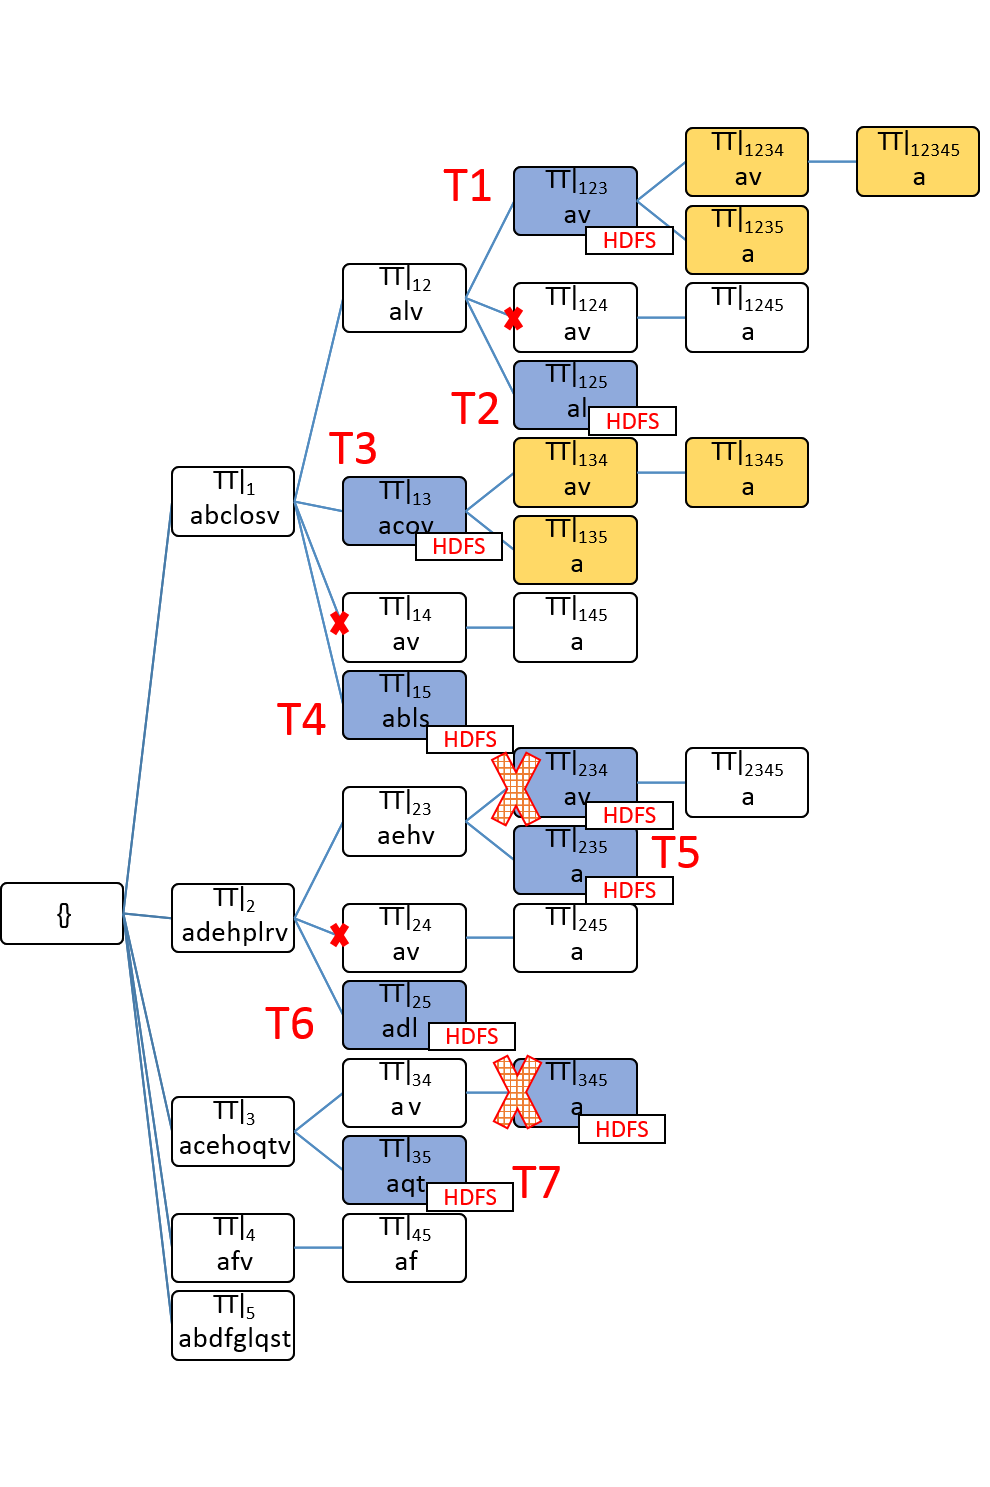
\includegraphics[width=4in]{chapters/pampa/running_example3_d_B_quadretti.png}
% where an .eps filename suffix will be assumed under latex,
% and a .pdf suffix will be assumed for pdflatex; or what has been declared
% via \DeclareGraphicsExtensions.
\caption{Execution of PaMPa-HD on the running example dataset.
For the sake of clarity, pruning rules 1 and 2 are not
applied. The big checked crosses on nodes represent the nodes which have been
removed by the synchronization job, e.g.,
the one on node \{2 3 4\} represents the pruning of node \{2 3 4\}.}
\label{running_3b}
\end{figure}

%Each worker node does not
%run Carpenter to the end but stops and writes intermediate results to the disk.
%After that, the redundancy is deleted with a synchronization job and Carpenter
%starts again from the filtered tables, handled in parallel by different tasks.

